\documentclass{article}
\usepackage{tikz}

\begin{document}

\centering

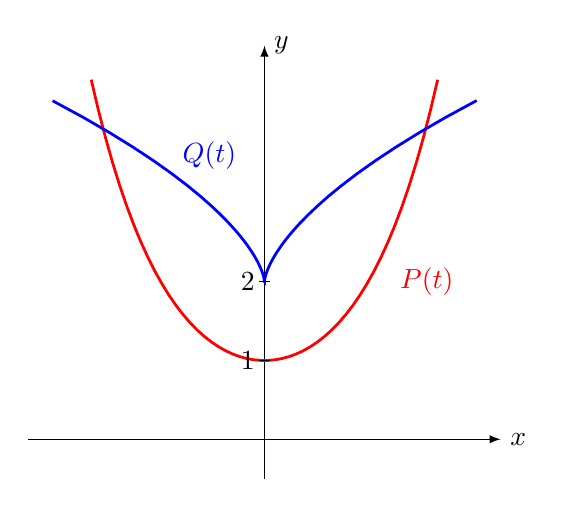
\begin{tikzpicture}
    % draw axes
    \coordinate (O) at (0,0);
    \draw[-latex] (0,-0.5) -- (0,5) node[anchor=west] {$y$};
    \draw[-latex] (-3,0) -- (3,0) node[anchor=west] {$x$};

    % draw curves
    \def\a{1} % constant
    \draw[red,domain=-2.2:2.2,samples=50, line width=1] plot ({\x},{\a*cosh(\x/\a)});
    \node[anchor=west] at (1.6,2) {\textcolor{red}{$P(t)$}};

    \draw[blue,domain=-1.4:1.4,samples=50, line width=1] plot ({\x - \a/2*sinh(2*\x/\a)},{2*\a*cosh(\x/\a)});
    \node[anchor = south] at (-0.7,3.3) {\textcolor{blue}{$Q(t)$}};

    % draw labels
    \node[anchor=east] at (0,2) {$2$};
    \draw (-2pt,2) -- (2pt,2);
    
    \node[anchor=east] at (0,1) {$1$};
    \draw (-2pt,1) -- (2pt,1);
    
\end{tikzpicture}
\end{document}